\subsection{Mikroprocessor}
\subsubsection{Arduino Mega 2560}
Som alternativ til at anvende UCN boardet, er et Arduino Mega 2560 board blevet brugt. Dette er gjort da der i videreudvikling benyttes shields som ikke er kompatibel med UCN boardet. Endvidere skal der bruges mere hukommelse til videreudviklingen, end UCN boardet har til rådighed.
\\
\\
Mikroprocessoren har 54 digitale pins og 14 analoge pins der fungerer som in- og output. Derudover har den 4 UART(Universal asynchronous receiver/transmitter) porte som anvedes til at kommunikere med microprocessorens interface.
\\
\\
Disse pins fungerer i spændingsintervallet 0-5 V. ATmega2560 er Arduino Mega's processor og kører med en krystal med en clockfrekvens på 16 MHz. Strømmen kan tilføres gennem USB, power jack eller gennem pin $V_{in}$ og anbefales en spænding mellem 7-12 V. 
\\
\\
Mikroprocessoren kan forbindes til computeren ved hjælp af USB, som gør det muligt for de to enheder at kommunikere med hinanden. Gennem USB forbindelsen kan softwaren overføres fra computeren til Arduinoen. Om nødvendigt kan chippen genstartes på mikroprocessoren gennem en resetknap, som er monteret på dens PCB(Printed Circuit Board).
\newline
\newline
Arduino Mega 2560 har den fordel at være kompatibel med standard bibliotekerne fra Arduino, hvorimod UCN boardet vil kræve at meget af softwaren, der benyttes til videreudviklingen, skal bygges fra bunden.

\begin{figure}[h!]
  \centering
  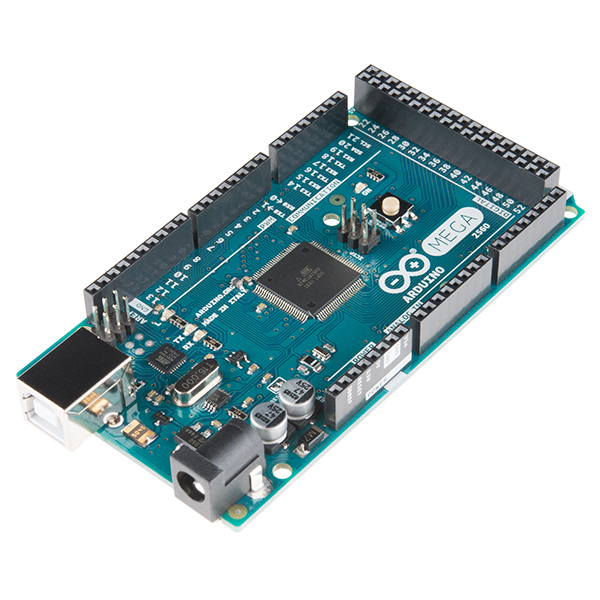
\includegraphics[width=0.7\textwidth]{figures/arduinoMega.jpg}
  \caption{Arduino Mega 2560. Foto af:  http://www.robotshop.com}
  \label{arduino2569}
\end{figure} 

\newpage



